Some students have encountered what might be called ``phantom interrupts'' when the system initially powers-up.
If your system is in Single Pulse mode when initially powered up, this could cause what appears to be an object detection despite not having pressed the button.
We'reno aware of this issue, and our plan during grading is to politely ignore it when that happens immediately upon starting the program.

If it bugs you enough, you can address it through the sensor’s state machine.

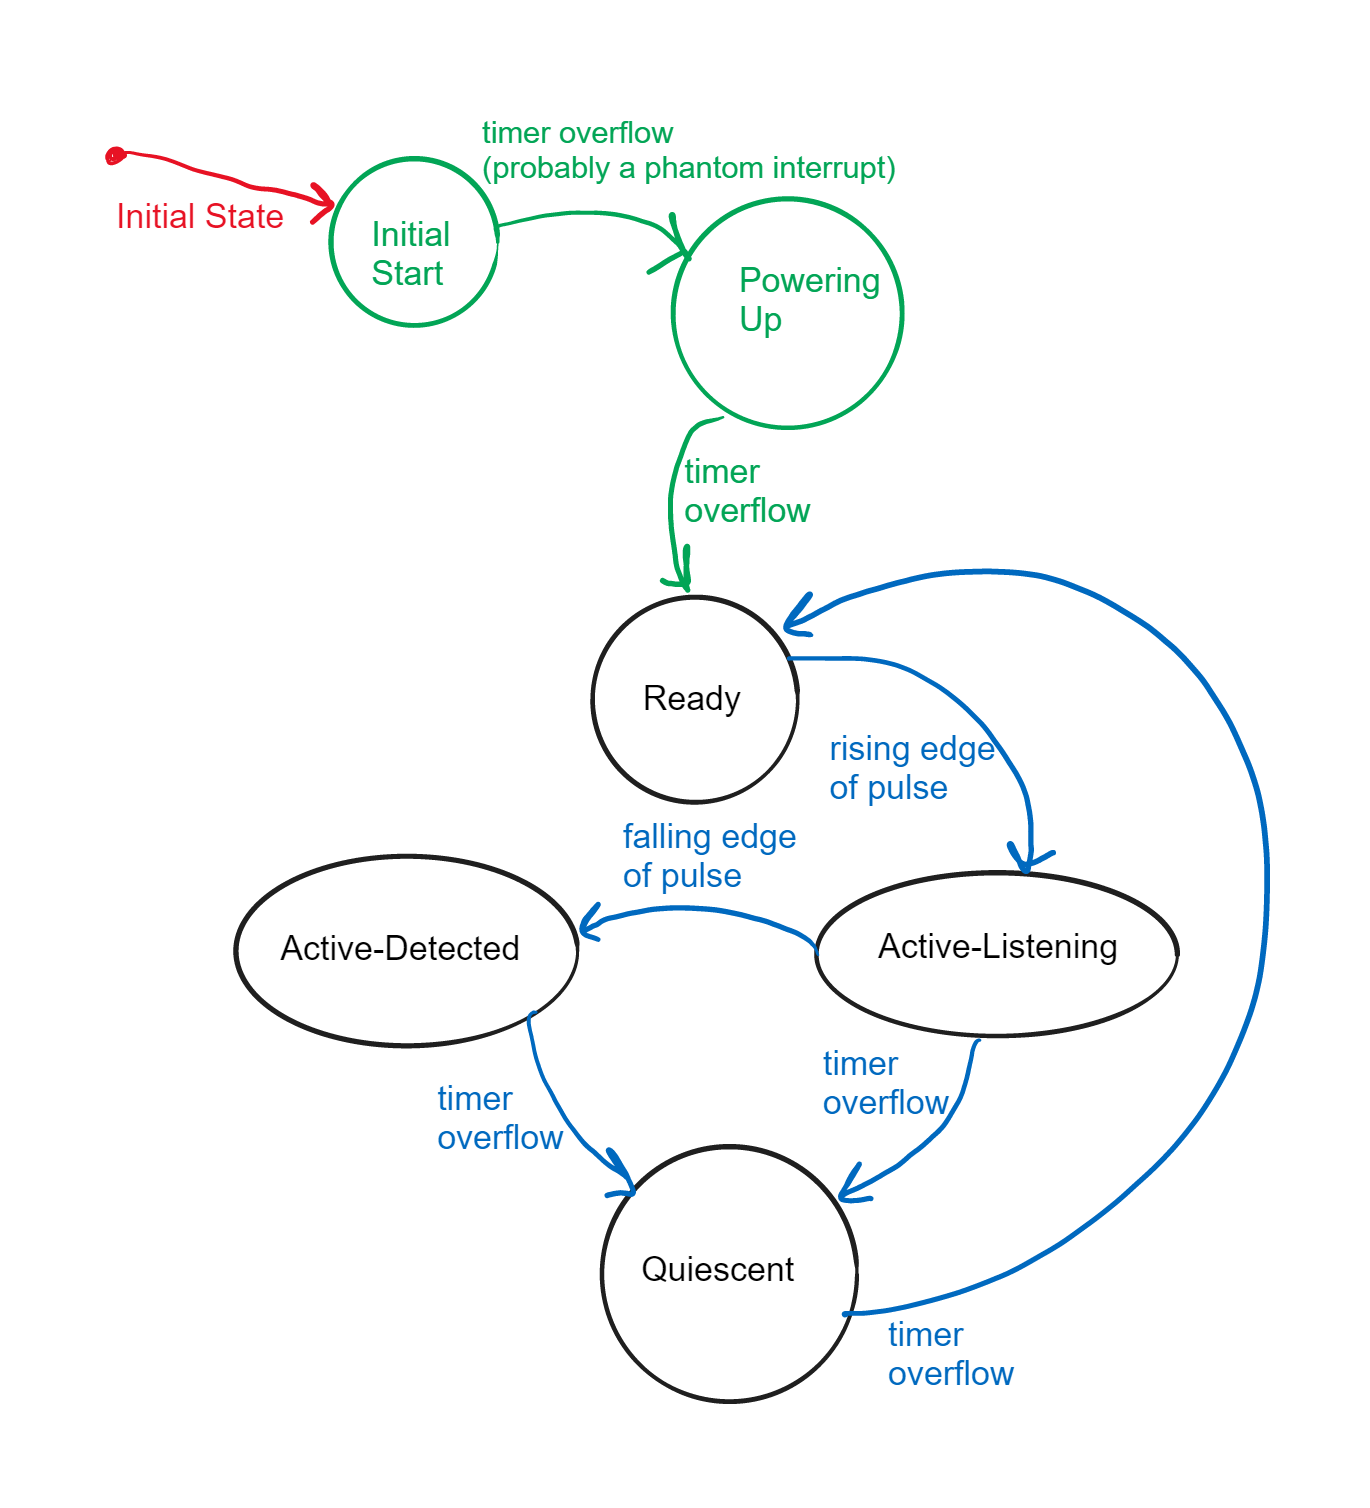
\includegraphics[width=4in]{noPhantomInterrupts}

Nothing happens in the ``Initial Start'' and ``Powering Up'' states – in fact, that’s the point of them.
If you only respond to pulse edges when you’re in the ``Ready'' state or the ``Active-Listening'' state, then phantom pin change interrupts that happen when powering-up the system won’t affect anything.
They’ll happen in the first few dozen nanoseconds, when your system is either in the ``Initial Start'' state or the ``Powering Up'' state.
(We don’t know whether the phantom pin change interrupt, if it happens, will occur before or after the phantom timer interrupt, if it occurs, which is why we have two do-nothing states.)